%\documentclass[pdf,final,colorBG,slideColor]{prosper}
\documentclass[xcolor=dvipsnames]{beamer}
%%\usetheme{default}
\usecolortheme[named=Maroon]{structure}
%\usetheme{Boadilla}
\usetheme{Madrid}
\useoutertheme{default}%[footline=empty]{infolines}

% \usepackage{helvet}
% \usepackage{enumerate}
% \usepackage{amsmath}
% \usepackage{amsfonts}
% \usepackage{graphicx}
% \usepackage{ulem}
% \usepackage{multirow}
\usepackage{comment}

\usepackage[absolute,overlay]{textpos}

%\RequirePackage{algorithmic}
%\RequirePackage{algorithm}
% \renewcommand{\algorithmicrequire}{\textbf{Inputs:}}
% \renewcommand{\algorithmicensure}{\textbf{Outputs:}}


%\newtheorem{theorem}{Theorem}
%\newtheorem{lemma}{lemma}
%\newtheorem{corollary}{Corollary}
%\newtheorem{proposition}{Proposition}
%\newtheorem{Q}{Question}
%\newtheorem{Exa}{Example}
%\newtheorem{Definition}{Definition}


\newcommand{\Fq}{{\mathbb{F}}_{q}}
\newcommand{\Fkk}{{\mathbb{F}}_{2^k}}
\newcommand{\Zkk}{{\mathbb{Z}}_{2^k}}
\newcommand{\Fkkx}[1][x]{\ensuremath{\mathbb{F}}_{2^k}[#1]\xspace}
\newcommand{\Grobner}{Gr\"{o}bner\xspace}
\newcommand{\bi}{\begin{itemize}}
\newcommand{\ei}{\end{itemize}}

\title[Verify GF Arithmetic with Gr\"obner Bases]{Formal 
Verification of   Galois Field Arithmetic Circuits using Computer
Algebra Techniques}



\author[P. Kalla]{Priyank Kalla}
%\email{rostamian@umbc.edu}
\institute[Univ. of Utah]{
\includegraphics[height=17mm]{/Users/Kalla/teaching/Comp-Algebra-Course/lectures/old_ulogo.eps}\\
\ \\
Associate Professor\\
Electrical and Computer Engineering, University of Utah\\
kalla@ece.utah.edu\\
\url{http://www.ece.utah.edu/~kalla}
}


\date{}
%\slideCaption{}

%% Images
\pgfdeclareimage[width=.4in]{fg:logo}{/Users/Kalla/teaching/Comp-Algebra-Course/lectures/old_ulogo.eps} 

%%%%%%%%%%%%%%%%%%%%%%%%%%%%%%%%%%%%%%%%%%%%%%%%%%
%%%%%%%%%%%%%%%%%%%%%%%%%%%%%%%%%%%%%%%%%%%%%%%%%%
%%%%%%%%%%%%%%%%%%%%%%%%%%%%%%%%%%%%%%%%%%%%%%%%%%
\begin{document}


%----------- titlepage ----------------------------------------------%
\begin{frame}[plain]
  \titlepage

\end{frame}

%\maketitle

%%%%%%%%%%%%Try section
% \section*{Outline}
% \begin{frame}

% \tableofcontents
% \end{frame}

% \section{Intro}
% \subsection{What's that?}
% \subsection{Overview of something}

% \section{Galois Fields}
% \subsection{what does this give?}
% \begin{frame}
% \end{frame}

%%%%%%%%%%

%%%%%%%%%%%%%%%%%%%%%%%%%%%%%%%%%%%%%%%%%%%%%%%%%%
\begin{frame}{\large{Some Background...}}

\begin{itemize}
\item My interests -- Design Automation and Verification
	\begin{itemize}
	\item Formal Verification of RTL-descriptions
        \item Word-level abstractions from designs, symbolic
          techniques
        \item Verification of finite-precision arithmetic
	\end{itemize}
\item Equivalence check: specification ({\it Spec}) vs implementation
  ({\it Impl})
	\begin{itemize}
	\item RTL-1 \& RTL-2: same function?
        \item  Word-level spec (polynomial, RTL) vs
          gate-level circuit: same function?
        \item RTL: functions over \alert{$k$-bit-vectors}
          \begin{itemize}
            \item $k$-bit-vector $\mapsto$ integers $\pmod{ 2^k} = \Zkk$
            \item $k$-bit-vector $\mapsto$ Galois (Finite) field $\Fkk$
          \end{itemize}
	\end{itemize}
\item Approach: {\bf Computer Algebra Techniques}
	\begin{itemize}
	\item  Model: Polynomial functions over $\Zkk$ or $\Fkk$
        \item  Devise decision procedures for polynomial function equivalence
        \item  Commutative algebra, algebraic geometry + contemporary
          verification
	\end{itemize}
\item This talk, mostly about verification over Galois fields
\end{itemize}
\end{frame}

%%%%%%%%%%%%%%%%%%%%%%%%%%%%%%%%%%%%%%%%%%%%%%%%%%
\begin{frame}{\large{My Collaborators}}

\begin{itemize}
\item Former PhD students
	\begin{itemize}
	\item Namrata Shekhar: Synopsys, Formality Equivalence Checker
        \item Sivaram Gopalakrishnan: Synopsys, Formality Equivalence Checker
        \item Jinpeng Lv: Cadence, Conformal Equivalence Checker
	\end{itemize}
\item Collaborator: Prof. Florian Enescu
	\begin{itemize}
	\item Mathematics \& Statistics, Georgia State Univ.
        \item Commutative Algebra \& Algebraic Geometry
        \item NOT a computer-algebra specialist, but thats good!
          \begin{itemize}
            \item Think about problems ``theoretically'', algorithms
              can come later...
          \end{itemize}
	\end{itemize}
\end{itemize}
\end{frame}



%%%%%%%%%%%%%%%%%%%%%%%%%%%%%%%%%%%%%%%%%%%%%%%%%%


\begin{frame}{\large{Agenda: Verification of Galois field circuits}}

\begin{itemize}
\item Motivation
	\begin{itemize}
	\item Galois fields, hardware applications \& their verification
	\end{itemize}
\item Target problems 
	\begin{itemize}
	\item Given Galois field $\Fkk$, polynomial $f$, and circuit $C$
        \item Verify: circuit $C$ implements $f$; or find the bug
        \item Given circuits $C_1, C_2$, is $C_1 \equiv C_2$ over
          $\Fkk$?
        \item Given circuit $C$, with $k$-bit inputs and outputs
          \begin{itemize}
            \item Derive a polynomial representation for $C$ over $f:
              \Fkk \rightarrow \Fkk$ 
              \item \alert{Word-level abstraction} as a canonical
                polynomial representation
          \end{itemize}
	\end{itemize}
\item Approach: {\bf Computer Algebra Techniques}
	\begin{itemize}
	\item  Nullstellensatz + Gr\"obner Basis methods
        \item  Challenge: Complexity of Gr\"obner Basis algorithm
        \item  Contribution: A {\bf term order} to {\bf obviate} the
          Gr\"obner Basis algorithm for verification + custom
          $F_4$-style reduction
	\end{itemize}
\item Results \& Conclusions
\end{itemize}
\end{frame}


%%%%%%%%%%%%%%%%%%%%%%%%%%%%%%%%%%%%%%%%%%%%%%%%%%
\begin{frame}{\large {Motivation}}
\vspace{-0.2in}
%\ptsize{10}

\begin{itemize}
\item Wide applications of Galois field circuits
	\begin{itemize}
	\item \textbf {Cryptography}: RSA, Elliptic
          Curve Cryptography (ECC) 
	\item Error Correcting Codes, Digital Signal Processing, etc.
	\end{itemize}	
\end{itemize}

\bi
\item Bugs in hardware can leak secret keys [{\it Biham et al.}, ``Bug
  Attacks'', Crypto 2008] 
\ei

% \begin{itemize}
% \item Type of circuits in ECC
% 	\begin{itemize}
% 	\item Multiplication dominates Galois field computations
% 	\item In cryptography: $99\%$ time in encryption and decryption
% 	\item 
% 	\end{itemize}
% \end{itemize}	

 \begin{itemize}
 \item Data-path size in ECC crypto-systems can be very large
 	\begin{itemize}
        \item In $\mathbb{F}_{2^k}$, $k = 163, 233, \dots$ (NIST standard)
        \item ECC-point addition for encryption, decryption, authentication
 	\item Custom arithmetic architectures -- hard to verify
        \item Synthesized circuits are ``easier'' to verify
 	\end{itemize}
 \end{itemize}

\begin{itemize}
\item Why use computer algebra?
	\begin{itemize}
        \item Algebraic nature (finite field) of the computation (polynomial)
	\item  Verification infeasible with contemporary verification tools 
	\end{itemize}
\end{itemize}

\end{frame}
%%%%%%%%%%%%%%%%%%%%%%%%%%%%%%%%%%%%%%%%%%%%%%%%%%
%%%%%%%%%%%%%%%%%%%%%%%%%%%%%%%%%%%%%%%%%%%%%%%%%%
\begin{frame}{\large {Galois Field Overview}}
%\vspace{-0.2in}
%\ptsize{10}
\textbf {Galois field} $\mathbb{F}_q$ is a finite field with $q$
elements, $q = p^k$
\begin{itemize}
\item Commutative Ring with unity, associate, distributive laws
\item Closure property: $+,-,\times$, inverse ($\div$)
\end{itemize}

\begin{itemize}
\item $\mathbb{F}_p \equiv (\mathbb{Z} ~\pmod{ p })$, where $p = $ prime, is a field
\begin{itemize}
\item $\mathbb{Z}_7=\{0,1,2,3,4,5,6\}$
\end{itemize}

% %\begin{comment}
% \item Ring $\mathbb{Z}_{2^k}$ ($k$-bit integer datapaths) are {\bf not} fields : 
% \begin{itemize}
% \item $\mathbb{Z}_{8}$, $\mathbb{Z}_{2^{32}}$ are not fields:
%   even numbers have no inverses
% %\item $\mathbb{R, Q, C}$ are infinite fields
% \end{itemize}
% %\end{comment}

\end{itemize}

Our interest: $\mathbb{F}_{q} = \mathbb{F}_{2^k}$, i.e. $q = 2^k$
\begin{itemize}
\item  $\mathbb{F}_{2^k}$: $k$-dimensional extension of  $\mathbb{F}_{2}$
	\begin{itemize}
	\item $k$-bit bit-vector, AND/XOR arithmetic
	\end{itemize}
\end{itemize}

To construct $\mathbb{F}_{2^k}$
\begin{itemize}
\item $\mathbb{F}_{2^k} \equiv \mathbb{F}_{2}[x] \pmod {P(x)}$
\item $P(x) \in \mathbb{F}_{2}[x]$, irreducible polynomial of degree $k$
\end{itemize}

\end{frame}
%%%%%%%%%%%%%%%%%%%%%%%%%%%%%%%%%%%%%%%%%%%%%%%%%%
%%%%%%%%%%%%%%%%%%%%%%%%%%%%%%%%%%%%%%%%%%%%%%%%%%
%\begin{comment}

\begin{frame}{Field Elements: {\it e.g.} $\mathbb{F}_8$}
%\ptsize{10}

Consider: $\mathbb{F}_{2^3}= \mathbb{F}_{2}[x] \pmod {x^3 + x +
  1}$\\ $A \in \mathbb{F}_{2}[x]$ \\ 
$A \pmod {x^3 + x + 1} = a_2 x^2 + a_1 x + a_0$. Let $P(\alpha) = 0$:

\begin{itemize}
\item $\langle a_2, a_1, a_0 \rangle = \langle 0, 0, 0\rangle = 0$
\item $\langle a_2, a_1, a_0 \rangle = \langle 0, 0, 1\rangle = 1$
\item $\langle a_2, a_1, a_0 \rangle = \langle 0, 1, 0\rangle = \alpha$
\item $\langle a_2, a_1, a_0 \rangle = \langle 0, 1, 1\rangle = \alpha
  + 1$
\item $\langle a_2, a_1, a_0 \rangle = \langle 1, 0, 0\rangle = \alpha^2$
\item $\langle a_2, a_1, a_0 \rangle = \langle 1, 0, 1\rangle =
  \alpha^2 + 1$
\item $\langle a_2, a_1, a_0 \rangle = \langle 1, 1, 0\rangle =
  \alpha^2 + \alpha$
\item $\langle a_2, a_1, a_0 \rangle = \langle 1, 1, 1\rangle =
  \alpha^2 + \alpha + 1$
\end{itemize}


\end{frame}

%\end{comment}

%%%%%%%%%%%%%%%%%%%%%%%%%%%%%%%%%%%%%%%%%%%%%%%%%%

\begin{frame}{{Elliptic Curves -- Point addition}}

%\ptsize{11}

\begin{center}
$y^2 + xy = x^3 + ax^2 + b$ over GF($2^k$)
\end{center}

\begin{columns}

\begin{column}{0.3\textwidth}
\begin{center}
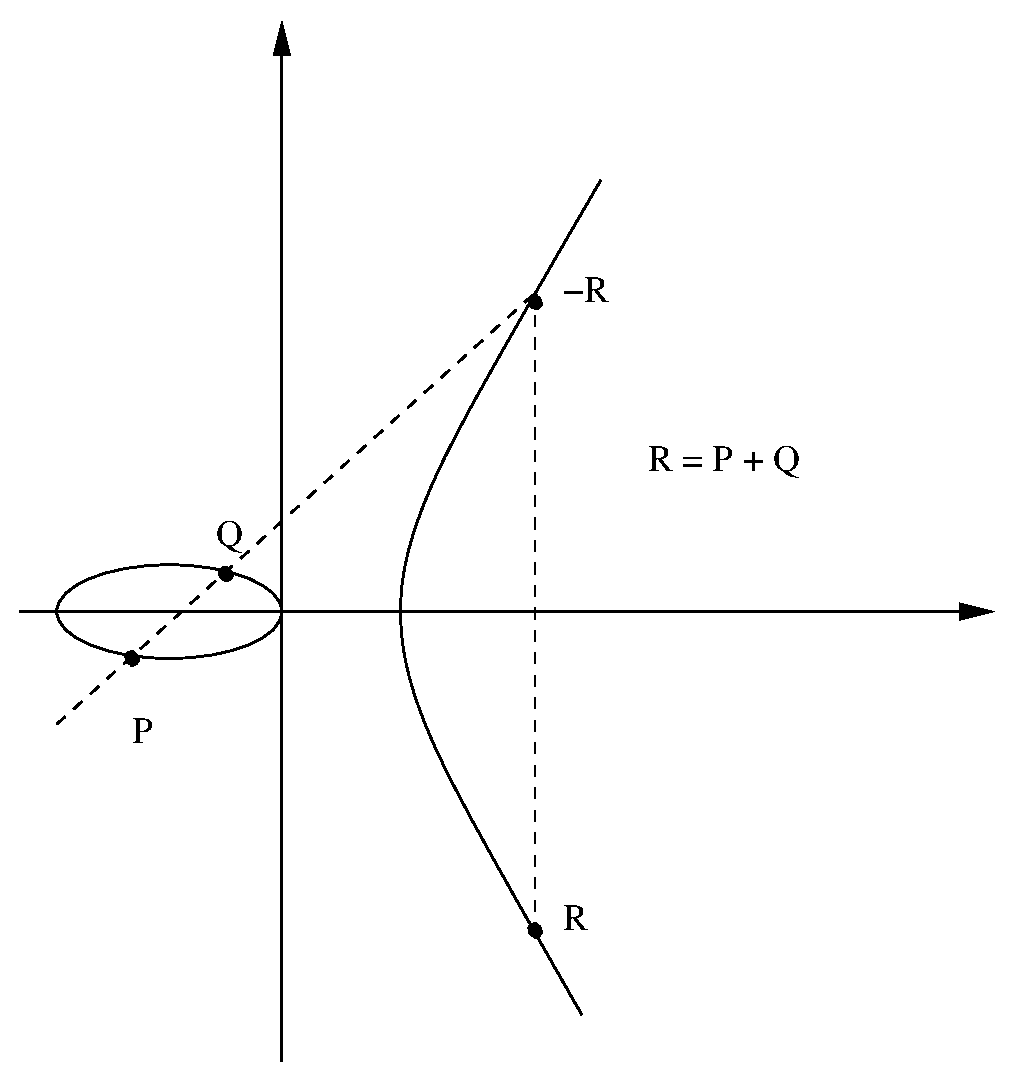
\includegraphics[height=50mm]{ecc.eps}
\end{center}
\end{column}
%%\end{minipage} \hfill \begin{minipage}[h]{3in}

\begin{column}{0.3\textwidth}
$$\text{Compute Slope:} {y_2 - y_1 \over x_2 - x_1}$$
Computation of inverses over $\Fkk$ is expensive
%\end{minipage}
\end{column}

\end{columns}
\end{frame}


%%%%%%%%%%%%%%


%%%%%%%%%%%%%%%%%%%%%%%%%%%%%%%%%%%%%%%%%%%%%%%%%%

\begin{frame}{{Point addition using Projective Co-ordinates}}

\begin{itemize}
\item Curve: ~~$Y^2 + XYZ = X^3Z + aX^2Z^2 + bZ^4$ over $\mathbb{F}_{2^k}$
\item Let ($X_3$, $Y_3$, $Z_3$) = ($X_1$, $Y_1$, $Z_1$) + ($X_2$,
  $Y_2$, $1$)  
\end{itemize}

\begin{columns}
\begin{column}{0.2\textwidth}
\begin{align*}
A &= Y_2 \cdot Z_1^2 + Y_1 \\
B &= X_2 \cdot Z_1 + X_1 \\
C &= Z_1 \cdot B \\
D &= B^2 \cdot(C + a Z_1^2) \\
\alert{Z_3} &= C^2 
\end{align*}
\end{column} 

\begin{column}{.3\textwidth}
\begin{align*}
E &= A \cdot C  \\
\alert{X_3} &= A^2 + D + E  \\
F &= X_3 + X_2 \cdot Z_3 \\
G &= X_3 + Y_2\cdot Z_3 \\
\alert{Y_3} &= E\cdot F + Z_3 \cdot G
\end{align*}
\end{column}
\end{columns}

\ \\
No inverses, just addition and multiplication

\end{frame}


%%%%%%%%%%%%%%


%%%%%%%%%%%%%%%%%%%%%%%%%%%%%%%%%%%%%%%%%%%%%%%%%%
\begin{frame}{Multiplication in GF($2^4$)}
%\ptsize{10}
Input: \\
$A=(a_3a_2a_1a_0)$ \\
$B=(b_3b_2b_1b_0)$ \\
$A=a_0+a_1\cdot \alpha+a_2\cdot \alpha^2+a_3\cdot \alpha^3$\\
$B=b_0+b_1\cdot \alpha+b_2\cdot \alpha^2+b_3\cdot \alpha^3$
\bigskip

Irreducible Polynomial: \\
$P=(11001)$ \\
$P(x)=x^4+x^3+1, ~~ P(\alpha) = 0$
\bigskip

Result: 

$A\times B \pmod{ P(x) }$


\end{frame}

%%%%%%%%%%%%%%%%%%%%%%%%%%%%%%%%%%%%%%%%%%%%%%%%%%
%%%%%%%%%%%%%%%%%%%%%%%%%%%%%%%%%%%%%%%%%%%%%%%%%%
\begin{frame}{Multiplication over GF($2^4$)}

 {\begin{tabular}{c c c c c c c c}
  &   &   & $a_3$ & $a_2$ & $a_1$ & $a_0$  \\ 
 $\times$&   &   & $b_3$ & $b_2$ & $b_1$ & $b_0$  \\ 
 \hline
 &   &   & $a_3\cdot b_0$ & $a_2 \cdot b_0$ & $a_1\cdot b_0$ & $a_0\cdot b_0$ \\
 &  & $a_3\cdot b_1$ & $a_2\cdot b_1$ & $a_1 \cdot b_1$ & $a_0\cdot b_1$ &   \\
 & $a_3\cdot b_2$ & $a_2\cdot b_2$ & $a_1\cdot b_2$ & $a_0\cdot b_2$ &  &   \\
 $a_3\cdot b_3$ & $a_2\cdot b_3$ & $a_1\cdot b_3$ & $a_0\cdot b_3$ &  &  &   \\
 \hline
 $s_6$& $s_5$  & $s_4$  & $s_3$ & $s_2$  & $s_1$   & $s_0$ 
 \end{tabular}\par}

\ \\
\ \\
In polynomial expression:\\
$S=s_0+s_1\cdot \alpha+s_2\cdot \alpha^2+s_3\cdot \alpha^3+s_4\cdot \alpha^4+s_5\cdot \alpha^5+s_6\cdot \alpha^6$

\bigskip

$S$ should be further reduced $\pmod {P(x)}$
\end{frame}

%%%%%%%%%%%%%%%%%%%%%%%%%%%%%%%%%%%%%%%%%%%%%%%%%%
%%%%%%%%%%%%%%%%%%%%%%%%%%%%%%%%%%%%%%%%%%%%%%%%%%
\begin{frame}{Multiplication over GF($2^4$)}

 {\begin{tabular}{c c c| c c c c |c c c}
  $s_6$& $s_5$  & $s_4$  & $s_3$ & $s_2$  & $s_1$   & $s_0$ & &  \\
 \hline
 & & &$s_4$ & $0$&$0$ &$s_4$  &$\Leftarrow$ & $s_4\cdot \alpha^4 \pmod{ P(\alpha)}$\\
 & & &$s_5$ & $0$&$s_5$ &$s_5$ & $\Leftarrow$ & $s_5\cdot \alpha^5 \pmod{ P(\alpha)}$\\
 & &$+$ &$s_6$ & $s_6$&$s_6$ &$s_6$  & $\Leftarrow$ & $s_6\cdot \alpha^6
 \pmod{ P(\alpha)}$\\
 \hline
 & & & $g_3$ & $g_2$ &$g_1$ & $g_0$
 \end{tabular}\par}

\ \\

$s_4\cdot \alpha^4 \pmod {\alpha^3+\alpha+1}=s_4\cdot \alpha^3+s_4$ \\
$s_5\cdot \alpha^5 \pmod {\alpha^3+\alpha+1}=s_5\cdot \alpha^3+s_5\cdot \alpha+s_5$ \\
$s_6\cdot \alpha^6 \pmod {\alpha^3+\alpha+1}=s_6\cdot \alpha^3+s_6\cdot \alpha^2+s_6\cdot \alpha+s_6$ 
\bigskip

$G=g_0+g_1\cdot \alpha+g_2\cdot \alpha^2+g_3\cdot \alpha^3$
\end{frame}

%%%%%%%%%%%%%%%%%%%%%%%%%%%%%%%%%%%%%%%%%%%%%%%%%%
%%%%%%%%%%%%%%%%%%%%%%%%%%%%%%%%%%%%%%%%%%%%%%%%%%

% \begin{frame}{\large {Other GF-Multiply Architectures}}

% %\ptsize{11}
% \begin{itemize}
% \item Montgomery Multipliers used for exponentiation
% \item $F = MM(A, B) = A \times B \times R^{-1} \pmod{ P(x)}$
% \item Overkill for computing $A\times B$, but much faster for
%   computing $A^{n}$.
% \end{itemize}

% \begin{center}
% 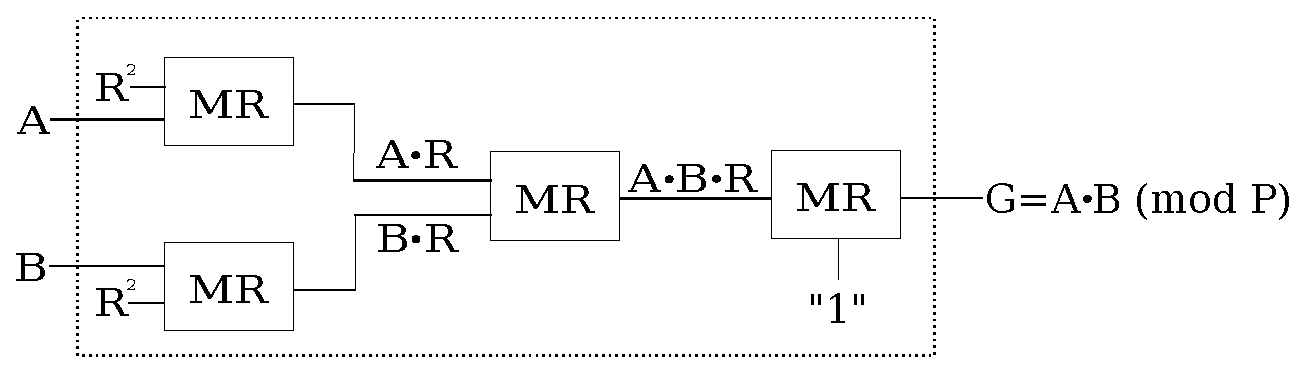
\includegraphics[height=30mm]{../VLSID2011/mmcircuit.eps}
% \end{center}

% \end{frame}


%%%%%%%%%%%%%%



%%%%%%%%%%%%%%%%%%%%%%%%%%%%%%%%%%%%%%%%%%%%%%%%%%
\begin{frame}{\large {Montgomery Architecture}}
%\vspace{-0.2in}
\begin{figure}[hbt]
\centerline{
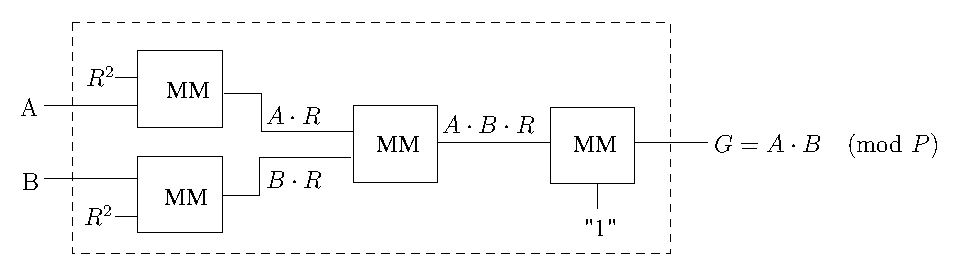
\includegraphics[scale=0.75]{mmcircuit.eps}
}
\caption{{\it Montgomery} multiplier over GF($2^k$)}
\label{fig:mm4}
\end{figure}

{{\it  Montgomery} Multiply: $F = A\cdot B \cdot R^{-1}$, $R = \alpha^k$}


\begin{itemize}
\item Barrett architectures do not require precomputed $R^{-1}$
\item We can verify $163$-bit circuits, and also catch bugs!
\item Conventional techniques fail beyond $16$-bit circuits
\end{itemize}


\end{frame}

%%%%%%%%%%%%%%%%%%%%%%%%%%%%%%%%%%%%%%%%%%%%%%%%%%

%%%%%%%%%%%%%%%%%%%%%%%%%%%%%%%%%%%%%%%%%%%%%%%%%%
\begin{frame}{\large {Verification: The Mathematical Problem}}
% \vspace{-0.2in}
% %\ptsize{10}

\begin{itemize}
\item Given \alert{specification polynomial}: $f: Z = A\cdot B \pmod{ P(x)}$
   over $\mathbb{F}_{2^k}$, for given $k$, and given $P(x)$,
   s.t. $P(\alpha) = 0$
\item Given \alert{circuit implementation} $C$
 \begin{itemize}
 \item Primary inputs: $A = \{a_0, \dots, a_{k-1}\}, B = \{b_0,
   \dots, b_{k-1}\}$
 \item Primary Output $Z = \{z_0, \dots, z_{k-1}\}$
 \item $A = a_0 + a_1 \alpha + a_2\alpha^2 + \dots + a_{k-1} \alpha^{k-1}$
 \item $  B = b_0 + b_1 \alpha + \dots + b_{k-1} \alpha^{k-1}, 
       ~Z = z_0 + z_1 \alpha + \dots + z_{k-1}$
 \end{itemize}
\item Does the circuit $C$ correctly compute specification $f$?
\end{itemize}

Mathematically:
\begin{itemize}
\item Model the circuit (gates) as polynomials $\{f_1, \dots, f_s\}
  \in \mathbb{F}_{2^k}[x_1, \dots, x_d]$
\item Do solutions to $f = 0$ (\alert{spec}) agree with solutions to
  $f_1 = f_2 = \dots = f_s = 0$ (\alert{implement})?
\item Does $f$ \alert{vanish} on the \alert{Variety} $V(f_1, \dots, f_s)$?
\end{itemize}
% \begin{itemize}
% \item If solutions exists: BUG! Otherwise, equivalence is proven
% \item SAT/SMT solvers: Search for a solution, solve systems of equations
% \item In Cryptography, $GF(2^k), k = 256$ or more
% \item SAT/SMT is infeasible. Can only solve at most $k = 16$.
% \end{itemize}

% \end{itemize}
% Our Approach: Use symbolic computer algebra and algebraic geometry to
% reason whether a given system of polynomials has a solution or not? 

\end{frame}

%%%%%%%%%%%%%%%%%%%%%%%%%%%%%%%%%%%%%%%%%%%%%%%%%%
\begin{frame}{Example Formulation}

\begin{figure}[hbt]
\centerline{
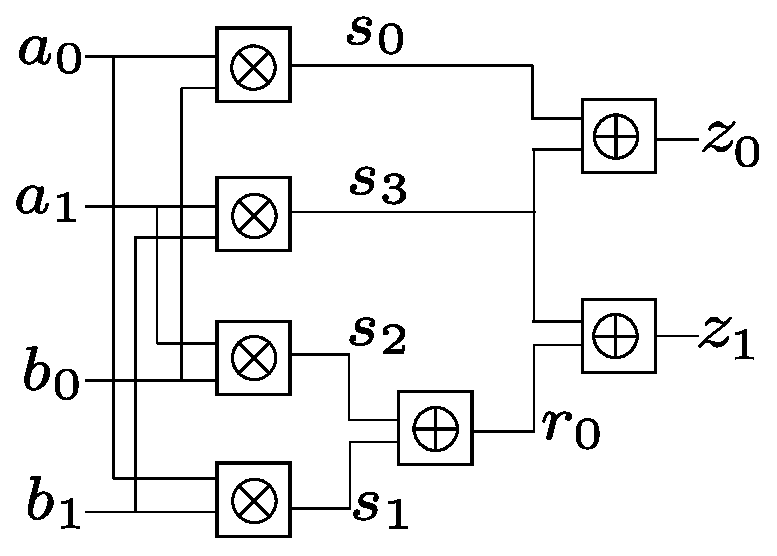
\includegraphics[scale=0.4]{2bitmultiplier.eps}
}
%\caption{A multiplier over GF($2^2$)}
\label{fig:mult-2-bit}
\end{figure}

Model circuit as polynomials in $\mathbb{F}_2 \subset \mathbb{F}_{2^k}$:
\begin{eqnarray}
z_0 = s_0 + s_3 ~~~~ \implies ~~~~ f_1: z_0 + s_0 + s_3 \nonumber\\
s_0 = a_0\cdot b_0 ~~~~ \implies ~~~~ f_2: s_0 + a_0\cdot b_0 \nonumber\\
\vdots\nonumber\\
A + a_0 + a_1\alpha, ~~B + b_0 + b_1\alpha, ~~Z + z_0 + z_1\alpha \nonumber
\end{eqnarray}
\end{frame}
%%%%%%%%%%%%%%%%%%%%%%%%%%%%%%%%%%%%%%%%%%%%%%%%%%

%%%%%%%%%%%%%%%%%%%%%%%%%%%%%%%%%%%%%%%%%%%%

%%%%%%%%%%%%%%%%%%%%%%%%%%%%%%%%%%%%%%%%%%%%%%%%%%
\begin{frame}{\large{Computer Algebra Terminology}}
\vspace{-0.2in}
%\ptsize{10}
Let $\mathbb{F}_q = GF(2^k)$:
\begin{itemize}
\item $\mathbb{F}_q[x_1, \ldots, x_n]$: ring of all polynomials with
  coefficients in $\mathbb{F}_q$ 
\item Given a set of polynomials:
\begin{itemize}
\item $f, f_1, f_2, \dots , f_s \in \mathbb{F}_q[x_1, \dots, x_n]$
\item Find solutions to $f_1 = f_2 = \dots = f_s = 0$
\end{itemize}
\item \alert{Variety:} Set of ALL solutions to a given system of polynomial equations: $V(f_1, \dots, f_s)$
	\begin{itemize}
	\item In $\mathbb{R}\left[x,y\right]$, $V(x^2+y^2-1)=\{all\  points\  on\ circle: x^2+y^2-1=0\}$
	\item In $\mathbb{R}[x]$, $V(x^2+1)=\emptyset$
	\item In $\mathbb{C}[x]$, $V(x^2+1)=\{(\pm i)\}$
	\end{itemize}
%\item Our Problem: Is the variety empty, i.e. is $V(f_1, \dots, f_s)
%=   \emptyset$ over $\mathbb{F}_q$? 
\item Variety depends on the \alert{ideal} generated by the polynomials.
\item Reason about the Variety by analyzing the Ideals
\end{itemize}


\end{frame}
%%%%%%%%%%%%%%%%%%%%%%%%%%%%%%%%%%%%%%%%%%%%%%%%%%
%%%%%%%%%%%%%%%%%%%%%%%%%%%%%%%%%%%%%%%%%%%%%%%%%%

\begin{frame}{\large {Ideals in Rings}}
\vspace{-0.2in}
%\ptsize{10}


% \begin{Definition}
% A subset $I \subset R = \mathbb{F}_q[x_1, \dots, x_n]$ is an \textbf {ideal} if:
% \begin{itemize}
% \item $0 \in I$
% \item If $f, g \in I$, then $f + g \in I$
% \item If $f \in I$ and $h \in R$ then $f \cdot h \in I$
% \end{itemize}
% \end{Definition}

\begin{Definition}
{\bf Ideals of Polynomials:} Let $f_1, f_2, \ldots, f_s \in
\mathbb{F}_q[x_1, \dots, x_n]$. Let 
\begin{eqnarray}
J = \langle f_1, f_2 \ldots, f_s\rangle = \{f_1 h_1 + f_2 h_2 + \dots + f_s h_s\} \nonumber 
\end{eqnarray}

$J = \langle f_1, f_2 \ldots, f_s\rangle$ is an ideal generated by
$f_1, \ldots, f_s$ and the polynomials are called the generators. 
\end{Definition}


\begin{Definition}
{\bf Ideal Membership:} Let $f, f_1, f_2, \ldots, f_s \in
\mathbb{F}_q[x_1, \dots, x_n]$. Let $J = \langle f_1, f_2 \ldots,
f_s\rangle$ be an ideal $\subset \mathbb{F}_q[x_1, \dots, x_n]$. 

If $f = f_1 h_1 + f_2 h_2 + \dots + f_s h_s$, then $f \in J$. 
\end{Definition}

If $f$ is a member of the ideal $J = \langle f_1, f_2 \ldots,
f_s\rangle$, then $f$ agrees with solutions of $f_1 = \dots = f_s = 0$.
\end{frame}

%%%%%%%%%%%%%%%%%%%



%%%%%%%%%%%%%%%%%%%%%%%%%%%%%%%%%%%%%%%%%%%%%%%%%%
\begin{frame}{Example Formulation}

\begin{figure}[hbt]
\centerline{
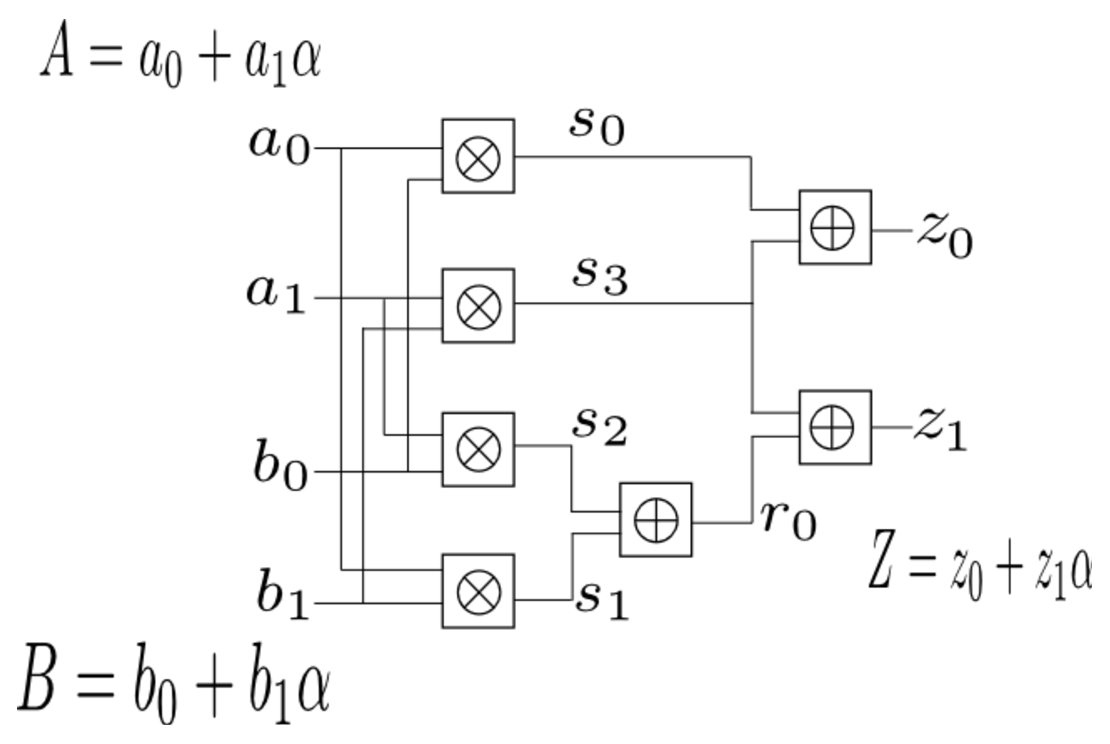
\includegraphics[scale=0.4]{drawing.eps}
}
%\caption{A multiplier over GF($2^2$)}
\label{fig:mult-2-bit}
\end{figure}

\begin{itemize}
\item Polynomials for all the gates: $f_1, \dots, f_s$; ideal $J =
  \langle f_1, \dots, f_s\rangle$
\item Polynomial specification: $f: Z = A\times B$
\item Spec $f$ ``agrees with'' all solutions to $f_1 = \dots = f_s = 0$
\item $f$ vanishes on variety $V_{\Fkk}(J)$?
\end{itemize}

\end{frame}
%%%%%%%%%%%%%%%%%%%%%%%%%%%%%%%%%%%%%%%%%%%%%%%%%%



%%%%%%%%%%%%%%%%%%%%%%%%%%%%%%%%%%%%%%%%%%%%%%%%%%

\begin{frame}{\large {Variety over $\mathbb{F}_q$ or over $\overline{\mathbb{F}_q}$?}}
Where are the solutions of $f_1 = f_2 = \cdots = f_s = 0$?

\begin{center}
    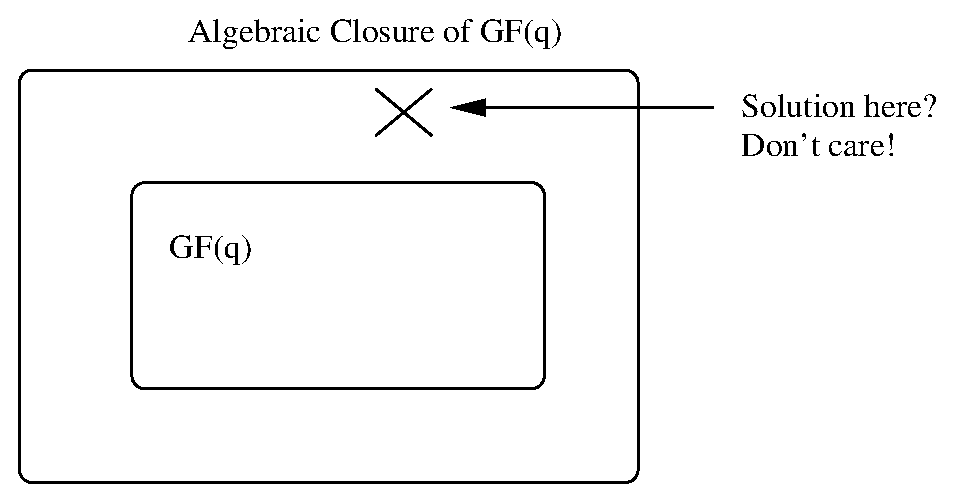
\includegraphics[scale=0.45]{gfq-closure.eps}
\end{center}

% \begin{itemize}
% \item Property of Finite fields: $\forall x\in \mathbb{F}_q,
%   x^q-x=0$
% \item {\bf Vanishing Polynomials: $x^q - x$} are vanishing polynomials
%   of $\mathbb{F}_q$
% \item Therefore $V(x^q - x) = \mathbb{F}_q$
% \end{itemize}

\begin{itemize}
\item \alert{Algebraically closed field} $\mathbb{F}$: Every $f(x) \in
  \mathbb{F}[x]$ has a root in $\mathbb{F}$
\item Galois fields are not algebraically closed!
\item $\overline{\mathbb{F}_q}$ = algebraic closure of $\mathbb{F}_q$:
  $\overline{\mathbb{F}_q} \supset \mathbb{F}_q$

\begin{itemize}
\item Similar to $\mathbb{C} \supset \mathbb{R}$
\end{itemize}

\end{itemize}

\end{frame}
%%%%%%%%%%%%%%%%%%%%%%%%%%%%%%%%%%%%%%%%%%%%%%%%%%

\begin{frame}{\large {Restricting the Variety to $\mathbb{F}_q$?}}

\begin{center}
    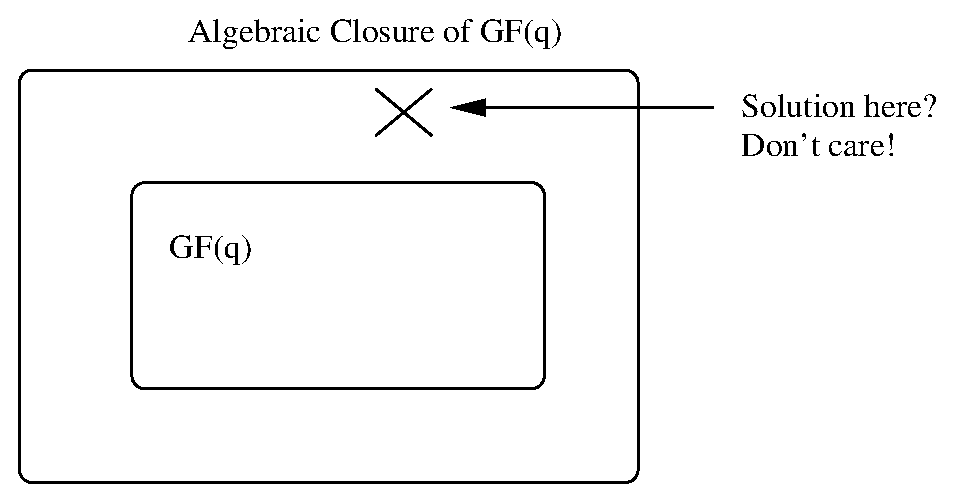
\includegraphics[scale=0.45]{gfq-closure.eps}
\end{center}

 \begin{itemize}
 \item Property of Finite fields: $\forall x\in \mathbb{F}_q, x^q-x=0$
 \item {\bf Vanishing Polynomials: $x^q - x$} are vanishing polynomials
   of $\mathbb{F}_q$
 \item Therefore $V(x^q - x) = \mathbb{F}_q$
 \item Restrict the solutions to $\mathbb{F}_q$: $V_{\mathbb{F}_q}(f_1, \dots, f_s) =
   V_{\overline{\mathbb{F}_q}}(f_1, \dots, f_s, ~~x_1^q - x_1, \dots,  x_n^q - x_n)$
 \end{itemize}


\end{frame}



%%%%%%%%%%%%%%%%%%%%%%%%%%%%%%%%%%%%%%%%%%%%%%%%%%
\begin{frame}{\large {Our Problem Formulation (Finally!)}}

Given $f$ (spec) and $f_1, \dots, f_s$ (circuit) over
  $\mathbb{F}_q[x_1, \dots, x_n]$
\begin{itemize}
\item $J = \langle f_1, f_2 \ldots, f_s\rangle$, Polynomials from the design
\item $J_0 = \langle x_1^q  - x_1, \dots, x_n^q - x_n\rangle$,
  Vanishing polynomials generated
\item $J + J_0 = \langle f_1, f_2 \ldots, f_s, ~~ x_1^q
  - x_1, \dots, x_n^q - x_n\rangle$;  Variety $V(J + J_0) = $ circuit configuration
\item Is $f \in J + J_0$? If so, the circuit is correct. Otherwise
  there is a bug.
\item This result is derived from \alert{Strong Nullstellensatz} over $\mathbb{F}_q$
\end{itemize}

\ \\
% Recall: If $f = f_1 h_1 + f_2 h_2 + \dots + f_s h_s$, then $f
%   \in \langle f_1, \dots, f_s\rangle$
% \begin{itemize}
% \item To test if $f \in \langle f_1, \dots, f_s\rangle$? Intuitively,
% \item Divide $f \stackrel{f_1, f_2, \cdots,
%     f_s}{\textstyle\longrightarrow}_+r$. If $r = 0 \implies f
%   \in \langle f_1, \dots, f_s\rangle$.
% \item But what if $r\neq 0$? $f$ may still be in the ideal!

% \end{itemize}

% Need a complete decision procedure....

If $f$ vanishes on $V_{\Fq} (J)$, then:\\
\begin{center}
 $f \in I(V_{\Fq}(J)) = I(V_{\overline{\Fq}}(J + J_0)) = \sqrt{J +
   J_0} = J + J_0$\\
\ \\
Our problem: Test of $f \in (J + J_0)$\\

Requires the computation of a \alert{Gr\"obner basis of $J + J_0$}
\end{center}
\end{frame}

%%%%%%%%%%%%%%%%%%%%%%%%%%%%%%%%%%%%%%%%%%%%%%%%%%
\begin{frame}{\large {Ideal Membership Test Requires a Gr\"obner Basis}}
\vspace{-0.2in}
%\ptsize{10}

\begin{itemize}
\item Different generators can generate the same ideal
\item $\langle f_1,\cdots,f_s \rangle=\cdots=\langle g_1,\cdots,g_t
  \rangle$
\item Some generators are a ``better'' representation of the ideal
\item A {\bf Gr\"obner basis} is a ``canonical'' representation of an ideal
\end{itemize}

Given $F = \{f_1, f_2,\cdots, f_s\}$, Compute a Gr\"obner Basis $G =
\{g_1,g_2,\cdots,g_t\}$, such that $I = \langle F \rangle = \langle G \rangle$

\begin{center}
$V(F)=V(G)$
\end{center}

Grobner Basis $G$ decides ideal membership:\\
\begin{center}
$G = GB(I) \iff \forall f \in I, f \stackrel{g_1, g_2, \cdots,
  g_t}{\textstyle\longrightarrow}_+0$ 
\end{center}

\end{frame}

%%%%%%%%%%%%%%%%%%%%%%%%%%%%%%%%%%%%%%%%%%%%%%%%%%

\begin{frame}{\large{Buchberger's Algorithm Computes a Gr\"obner Basis}}

%{\small
%\begin{algorithm}
%\caption {Buchberger's Algorithm}
{\bf Buchberger's Algorithm}\\
%\label{alg:gb}
%\begin{algorithmic}
% \REQUIRE : $F = \{f_1, \dots, f_s\}$
 INPUT : $F = \{f_1, \dots, f_s\}$\\
% \ENSURE : $G = \{g_1,\dots ,g_t\}$\\ %, a Gr\"{o}bner basis \\
 OUTPUT : $G = \{g_1,\dots ,g_t\}$\\ %, a Gr\"{o}bner basis \\
  $G:= F$; \\
  REPEAT\\
  \hspace{0.1in} $G' := G$\\
  \hspace{0.1in} For each pair $\{f, g\}, f \neq g$ in $G'$ DO\\
\hspace{0.2in}  $S(f, g) \stackrel{G'}{\textstyle\longrightarrow}_+
r$ \\
\hspace{0.2in}  IF $r \neq 0$ THEN $G:= G \cup \{r\}$ \\
%\hspace{0.2in}  $G(x):=G(x) / x$
UNTIL $G = G'$
%\end{algorithmic}
%\end{algorithm}

\[
S(f,g)=\frac{L}{lt(f)}\cdot f - \frac{L}{lt(g)}\cdot g
\]
$L = \text{LCM}(lm(f), lm(g))$, ~~$lm(f)$: leading monomial of $f$
%}

\end{frame}

%%%%%%%%%%%%%%%%%%%%%%%%%%%%%%%%%%%%%%%%%%%%%%%%%%

\begin{frame}{\large Complexity of Gr\"obner Basis and Term Orderings}
%\ptsize{10}
\begin{itemize}
\item For $J \subset \mathbb{F}_q[x_1, \dots, x_n]$, Complexity
  $GB(J + J_0): q^{O(n)}$
\item GB complexity very sensitive to {\bf term ordering}
\item A term order has to be imposed for systematic polynomial computation
\end{itemize}

Let $f = 2x^2yz + 3xy^3 - 2x^3$
\begin{itemize}
\item LEX $x> y> z$: ~~$f = {\bf -2x^3} + 2x^2yz + 3xy^3$
\item  DEGLEX $x>y>z$:  ~~$f = {\bf 2x^2yz} + 3xy^3 -2x^3$
\item DEGREVLEX $x>y>z$: ~~$f = {\bf 3xy^3} + 2x^2yz - 2x^3$
\end{itemize}
Recall, S-polynomial depends on term ordering:
\[
S(f,g)=\frac{L}{lt(f)}\cdot f - \frac{L}{lt(g)}\cdot g;
~~~~~~L = \text{LCM}(lm(f), lm(g))
\]

\end{frame}

%%%%%%%%%%%%%%%%%%
\begin{frame}{\large Effect of Term Orderings}

If $lm(f) \cdot lm(g) = LCM(lm(f), lm(g))$, 
then $S(f,g)\stackrel{G'}{\textstyle\longrightarrow}_+ 0.$\\
\ \\
{\small
LEX: $x_0 > x_1 > x_2 > x_3$
\begin{itemize}
\item $f=x_0 x_1+x_2$, $g=x_1x_2+x_3$
\item $lm(f) = x_0 x_1; ~~ lm(g) = x_1 x_2$
\item $S(f, g) \stackrel{G'}{\textstyle\longrightarrow}_+ x_0x_3 + x_2^2$
\end{itemize}

LEX: $x_3 > x_2 > x_1 > x_0$
\begin{itemize}
\item $f=x_2 + x_0 x_1$, $g=x_3 + x_1x_2$
\item $lm(f) = x_2; ~~ lm(g) = x_3$, $S(f, g) \stackrel{G'}{\textstyle\longrightarrow}_+ 0$
\end{itemize}
}

Problem: Find a ``term order'' that makes ALL $\{lm(f), ~lm(g)\}$ 
relatively prime.

\end{frame}
%%%%%%%%%%%%%%%%%%

\begin{frame}{\large For Circuits, such an order can be derived}

\centerline{
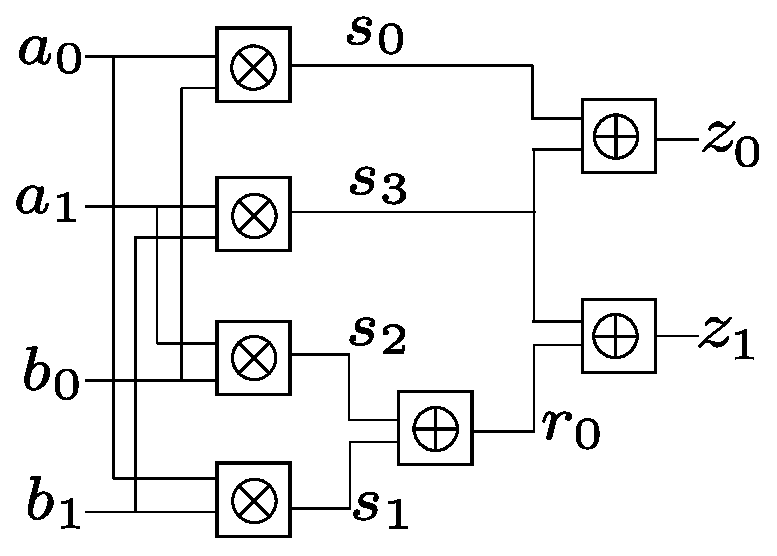
\includegraphics[scale=0.4]{2bitmultiplier.eps}
}
\vspace{-0.3in}
\begin{align*}
f_1: s_0+a_0 \cdot b_0, \ lm=s_0; ~~~f_2: s_1+a_0 \cdot b_1, \ lm=s_1 \nonumber \\
f_3: s_2+a_1 \cdot b_0, \ lm=s_2; ~~~f_4: s_3+a_1 \cdot b_1, \ lm=s_3 \nonumber \\
f_5: r_0+s_1 + s_2 , \ lm=r_0; ~~~f_6: z_0+s_0 + s_3, \ lm=z_0\nonumber
\end{align*}
\vspace{-0.3in}
\begin{center}
$f_7: z_1+r_0 + s_3, \ lm=z_1$ % \nonumber 
\end{center}

\begin{itemize}
\item Reverse Topological Traversal of the Circuit
\item $\{z_0 > z_1\} > \{r_0 > s_0 > s_3 \} > \{s_1 > s_2 \}> \{a_0 >
  a_1 >  b_0 > b_1\}$
\item Make every gate output a leading term
\end{itemize}

\end{frame}

%%%%%%%%%%%%%%%%%%%%%%%%%%%%%%%%%
\begin{frame}{\large{Our Discovery: Gr\"obner Basis of $J + J_0$}}

Using Our Topological Term Order:
\begin{itemize}
\item $F = \{ f_1, \dots, f_s\}$ is a Gr\"obner Basis of $J = \langle
  f_1, \dots, f_s\rangle$
\item $F_0 = \{x_1^q - x_1, \dots, x_n^q - x_n\}$ is also a Gr\"obner
  basis of $J_0$
\item But we have to compute a Gr\"obner Basis of $J + J_0 = \langle
  f_1, f_2 \ldots, f_s, ~~ x_1^q   - x_1, \dots, x_n^q - x_n\rangle$
\item We show that $\{f_1, f_2 \ldots, f_s, ~~ x_1^q   - x_1, \dots,
  x_n^q - x_n\}$ is a Gr\"obner basis!!
\item From our circuit: $f_i = x_i + P$
\item Only pairs to consider: $S(f_i, ~~~x_i^q - x_i)$ in Buchberger's Algorithm:
\end{itemize}

\[
S(f_i, ~~~x_i^q - x_i) \stackrel{J}{\textstyle\longrightarrow}_+ P^q -
P \stackrel{J_0}{\textstyle\longrightarrow}_+ 0
\]

Conclusion: Our term order makes $\{f_1, \dots, f_s, x_1^q - x_1,
\dots, x_n^q - x_n\}$ a Gr\"obner Basis
\end{frame}

%%%%%%%%%%%%%%%%%%%%%%%%%%%%%%%%%
\begin{frame}{\large Our Term Order: Already a Gr\"obner basis}

\centerline{
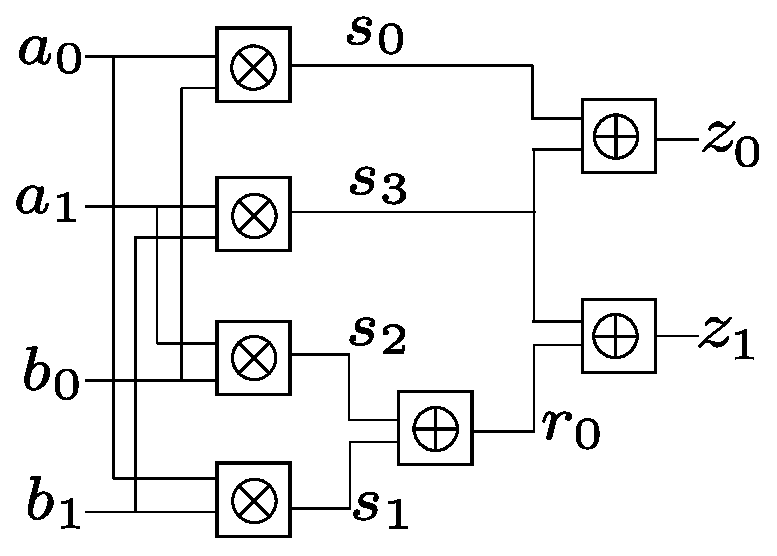
\includegraphics[scale=0.4]{2bitmultiplier.eps}
}
\vspace{-0.3in}
\begin{align*}
f_1: s_0+a_0 \cdot b_0, \ lm=s_0; ~~~s_0^q - s_0 \nonumber \\
f_2: s_2+a_1 \cdot b_0, \ lm=s_2; ~~~s_2^2 - s_2 \nonumber \\
\end{align*}
\vspace{-0.5in}

\begin{itemize}
\item Every gate: $f_i: x_i + P \in J$
\item Every vanishing polynomial: $x_i^q - x_i \in J_0$
\end{itemize}
$S(f_i, ~~~x_i^q - x_i) \stackrel{J}{\textstyle\longrightarrow}_+ P^q -
P \stackrel{J_0}{\textstyle\longrightarrow}_+ 0
$

$\{f_1, \dots, f_s, ~~x_1^q - x_1, \dots, x_n^q - x_n \}$  is a
Gr\"obner basis
\end{frame}



%%%%%%%%%%%%%%%%%%%%%%%%%%%%%%%%%%%%%%%%%%%%%%%%%%

\begin{frame}{Our  Overall Approach}

\begin{itemize}
\item Given the circuit, perform reverse topological traversal
\item Derive the term order to represent the polynomials for every gate
\item The set: $\{F, F_0\} = \{f_1, \dots, f_s, ~~x_1^q - x_1, \dots, x_n^q -
  x_n\}$ is a Gr\"obner Basis
\item Obtain: $f \stackrel{F, F_0}{\textstyle\longrightarrow}_+ r$
\item If $r = 0$, the circuit is correct
\item If $r \neq 0$, then $r$ contains only the \alert{primary input
    variables}
\item Any SAT assignment to $r\neq 0$ generates a counter-example
\item Counter-example found in no time as $r$ is simplified by Gr\"obner basis reduction
\end{itemize}

\end{frame}


%%%%%%%%%%%%%%%%%%%%%%%%%%%%%%%%%%%%%%%%%%%%%%%%%%

\begin{frame}{\large{Experimental Results: Correctness Proof}}
\vspace{-0.2in}
%\ptsize{8}

{\small
\begin{table}[h!]
\begin{center}
\caption{Verification Results of SAT, SMT, BDD, ABC. }
\begin{tabular}{|c||c|c|c|} \hline 
 & \multicolumn{3}{|c|}{Word size of the operands $k$-bits}\\ 
\hline
Solver & 8 & 12 & 16  \\
\hline \hline
MiniSAT& $22.55$& $TO$&$TO$  \\
\hline
CryptoMiniSAT &$7.17$&$16082.40$&$TO$  \\
\hline
PrecoSAT &$7.94$ &$TO$ &$TO$  \\
\hline
PicoSAT &$14.85$ &$TO$ &$TO$  \\
\hline \hline
Yices  &$10.48$ &$TO$ &$TO$ \\
\hline
Beaver &$6.31$ &$TO$ &$TO$  \\
\hline
CVC &$TO$ &$TO$ &$TO$  \\
\hline
Z3  &$85.46$ &$TO$ &$TO$ \\
\hline
Boolector &$5.03$&$TO$ &$TO$ \\
\hline 
Sonolar &$46.73$& $TO$ &$TO$  \\
\hline
SimplifyingSTP &$14.66$&$TO$ &$TO$  \\
\hline 
ABC &$242.78$&$TO$ &$TO$  \\
\hline \hline
BDD &$0.10$ &$14.14$ &$1899.69$  \\
\hline
\end{tabular}
\end{center}
\end{table}
}

\end{frame}

%%%%%%%%%%%%%%%%%%%%%%%%%%%%%%


\begin{frame}{\large{Experimental Results: Correctness Proof}}

\begin{table}[h!]
\begin{center}
\caption{\small Verify bug-free and buggy Mastrovito
  multipliers.  {\sc Singular} computer algebra
  tool used for division. }  
\label{tab:ours}
\begin{tabular}{|l||c|c|c|c|c|c|} \hline 
Size $k$-bits& 32  & 64 & 96 & 128  &160 &163\\
\hline
\#variables &$1155$ &$4355$ &$9603$ &$16899$ &$26243$ &$27224$ \\
\hline
\#polynomials &$1091$  &$4227$ &$9411$ &$16643$ &$25923$ &$26989$ \\
\hline
\#terms &$7169$  &$28673$ &$64513$ &$114689$ &$179201$ &$185984$ \\
\hline
Compute-GB:& $93.80$  & $MO$ &$MO$ &$MO$ &$MO$ &$MO$ \\
\hline
Ours: Bug-free&$1.41$ &$112.13$ &$758.82$ &$3054$ &$9361$ &$16170$ \\
\hline
Ours: Bugs& $1.43$  &$114.86$ &$788.65$ &$3061$  &$9384$ &$16368$\\
\hline
\end{tabular}
\end{center}
\end{table}


\end{frame}
%%%%%%%%%%%%%%%%%%%%%%%%%%%%%%


%%%%%%%%%%%%%%%%%%%%%%%%%%%%%%%%%
\begin{frame}{\large{Improve GB-reduction: $F_4$-style reduction}}

New algorithm to compute a Gr\"obner basis by J.C. Faug\`{e}re: $F_4$
\begin{itemize}
\item Buchberger's algorithm $S(f, g) \stackrel{G}{\textstyle\longrightarrow}_+
r$
\item Instead, compute a ``set'' of $S(f, g)$ in one-go
\item Reduces them ``simultaneously''
\item Significant speed-up in computing a Gr\"obner basis
\item Models the problem using \alert{sparse linear algebra}
\item Gaussian elimination on a matrix representation of the problem
\end{itemize}

Our term order: already a Gr\"obner basis. We only need $F_4$-style
reduction: $f \xrightarrow{F, F_0}_+r$
\end{frame}

%%%%%%%%%%%%%%%%%%%%%%%%%%%%%%

\begin{frame}{\large{$F_4$-style reduction}}

\bi
\item Spec: $f: Z + A\cdot B$, compute $f \xrightarrow{f_1, \dots, f_s}_+ r$
\item Find a polynomial $f_i$ that divides $f$, or ``cancels'' $LT(f)$
\item $Z = z_0 + z_1\alpha, ~~ A = a_0 + a_1\alpha, ~~ B = b_0 +
  b_1\alpha$
\item Construct a matrix: rows = polynomials, columns = monomials,
  entries = coefficient of monomial present in the polynomial
\ei


\begin{math}
\bordermatrix{
~ & Z  & AB & Ba_0 & Ba_1 & z_0 & z_1 & r_0 & a_0b_0 & a_0b_1 & a_1b_0& a_1b_1\cr
f & 1 &1 &0 &0 &0 &0 &0 &0 &0 &0 &0\cr
f_3 & 1 &0 &0 & 0 &1 &\alpha &0 &0 &0 &0 &0 \cr
Bf_1 & 0 &1 &1 &\alpha &0 &0 &0 &0 &0 &0 &0\cr
a_0f_2 &0  &0 &1 &0 &0 & 0& 0&1 &\alpha &0 &0\cr
a_1f_2 &0  &0 &0 &1 &0 &0 &0 &0 &0 &1 &\alpha\cr
f_5  & 0 &0 &0 &0 &1 &0 &0 &1 &0 &0 &1\cr
f_6  & 0 &0 &0 &0 &0 &1 &1 &0 &0 &0 &1\cr
f_4 & 0 &0 &0 &0 &0 &0 &1 &0 &1 &1 &0\cr
}
\end{math}

\end{frame}

%%%%%%%%%%%%%%%%%%%%%%%%%%%%%%



%%%%%%%%%%%%%%%%%%%%%%%%%%%%%%

\begin{frame}{\large{$F_4$-style reduction}}

\bi
\item Spec: $f: Z + A\cdot B$, compute $f \xrightarrow{f_1, \dots, f_s}_+ r$
\item $f_3: Z = z_0 + z_1\alpha$ %$Z + AB \xrightarrow{Z + z_0 + z_1 \alpha}_+r$
\ei

\begin{math}
\bordermatrix{
~ & \alert{Z}  & \alert{AB} & Ba_0 & Ba_1 & z_0 & z_1 & r_0 & a_0b_0 & a_0b_1 & a_1b_0& a_1b_1\cr
\alert{f} & \alert{1} &\alert{1} &0 &0 &0 &0 &0 &0 &0 &0 &0\cr
\alert{f_3} & \alert{1} &0 &0 & 0 &\alert{1} &\alert{\alpha} &0 &0 &0 &0 &0 \cr
Bf_1 & 0 &1 &1 &\alpha &0 &0 &0 &0 &0 &0 &0\cr
a_0f_2 &0  &0 &1 &0 &0 & 0& 0&1 &\alpha &0 &0\cr
a_1f_2 &0  &0 &0 &1 &0 &0 &0 &0 &0 &1 &\alpha\cr
f_5  & 0 &0 &0 &0 &1 &0 &0 &1 &0 &0 &1\cr
f_6  & 0 &0 &0 &0 &0 &1 &1 &0 &0 &0 &1\cr
f_4 & 0 &0 &0 &0 &0 &0 &1 &0 &1 &1 &0\cr
}
\end{math}

\end{frame}

%%%%%%%%%%%%%%%%%%%%%%%%%%%%%%



%%%%%%%%%%%%%%%%%%%%%%%%%%%%%%

\begin{frame}{\large{$F_4$-style reduction}}

\bi
\item To cancel the term \alert{$AB$}
\item $f_1: A = a_0 + a_1\alpha$ 
\item $Bf_1: AB = B a_0 + B a_1\alpha$
\ei

\begin{math}
\bordermatrix{
~ & Z  & \alert{AB} & Ba_0 & Ba_1 & z_0 & z_1 & r_0 & a_0b_0 & a_0b_1 & a_1b_0& a_1b_1\cr
{f} & {1} &\alert{1} &0 &0 &0 &0 &0 &0 &0 &0 &0\cr
{f_3} & {1} &0 &0 & 0 &{1} &{\alpha} &0 &0 &0 &0 &0 \cr
\alert{Bf_1} & 0 &\alert{1} &\alert{1} &\alert{\alpha} &0 &0 &0 &0 &0 &0 &0\cr
a_0f_2 &0  &0 &1 &0 &0 & 0& 0&1 &\alpha &0 &0\cr
a_1f_2 &0  &0 &0 &1 &0 &0 &0 &0 &0 &1 &\alpha\cr
f_5  & 0 &0 &0 &0 &1 &0 &0 &1 &0 &0 &1\cr
f_6  & 0 &0 &0 &0 &0 &1 &1 &0 &0 &0 &1\cr
f_4 & 0 &0 &0 &0 &0 &0 &1 &0 &1 &1 &0\cr
}
\end{math}

\end{frame}

%%%%%%%%%%%%%%%%%%%%%%%%%%%%%%

%%%%%%%%%%%%%%%%%%%%%%%%%%%%%%

\begin{frame}{\large{$F_4$-style reduction}}

\bi
\item Construct the Matrix for polynomial reduction
\item Apply Gaussian elimination on the matrix
\item Last row = result of reduction = $\alpha^2 + \alpha + 1 = 0$
\ei


\begin{math}
\bordermatrix{
~ & Z  & AB & Ba_0 & Ba_1 & z_0 & z_1 & r_0 & a_0b_0 & a_0b_1 & a_1b_0& a_1b_1\cr
& 1 &1 &0 &0 &0 &0 &0 &0 &0 &0 &0\cr
& 0 &1 &0 & 0 &1 &\alpha &0 &0 &0 &0 &0 \cr
& 0 &0 &1 &\alpha &1 &\alpha &0 &0 &0 &0 &0\cr
&0  &0 &0 &\alpha &1 & \alpha& 0&1 &\alpha &0 &0\cr
&0  &0 &0 &0 &1 &\alpha &0 &1 &\alpha &\alpha &\alpha^2\cr
& 0 &0 &0 &0 &0 &\alpha &0 &0 &\alpha &\alpha &\alpha^2+1\cr
& 0 &0 &0 &0 &0 &0 &\alpha &0 &\alpha &\alpha &\alpha^2+\alpha+1\cr
& 0 &0 &0 &0 &0 &0 &0 &0 &0 &0 &\alpha^2+\alpha+1\cr
}
\end{math}


\end{frame}

%%%%%%%%%%%%%%%%%%%%%%%%%%%%%%

\begin{frame}{Results}

\begin{table}[htb!]
\begin{center}
{\small
\caption{ Runtime for verifying bug-free and buggy Montgomery
  multipliers. TO = timeout of 10hrs. Time is given
  in seconds. $\ast$ denotes {\sc singular}'s capacity exceeded.} 
\label{tab:mmexp}
\begin{tabular}{|c||c|c|c|c|c|c|} \hline 
Operand size $k$ &  32 & 48 & 64 & 96 & 128 &163\\
\hline
\#variables     &$1194$     &$2280$     &$4395$     &$6562$     &$14122$  &$91246$\\
\hline
\#polynomials    &$1130$     &$2184$     &$4267$     &$6370$     &$13866$  &$89917$\\
\hline
\#terms          &$10741$    &$18199$    &$40021$    &$55512$    &$134887$ &$484738$\\
\hline \hline
Bug-free (Singular) &$1.50$  &$11.03$    &$27.70$    &$1802.75$  &$10919$   &$\ast$\\
\hline
Bug-free ($F_4$)   &$0.86$     &$4.47$     &$10.11$    &$700.59$   &$4539$    &$18374$\\
\hline \hline
Bugs (Singular)  &$1.52$     &$11.10$    &$28.18$    &$1812.15$  &$11047$   &$\ast$\\
\hline
Bugs ($F_4$)       &$0.88$     &$4.49$     &$10.12$    &$709.03$   &$4564$    &$17803$\\
\hline
\end{tabular}
}
\end{center}
\end{table}

$F_4$-style reduction 2.5X faster than use of Singular

\end{frame}

%%%%%%%%%%%%%%%%%%%%%%%%%%%%%%
\begin{frame}{Prior Work}

Wienand {\it et al} CAV'2008: Similar approach for verification
  of integer multipliers
\begin{itemize}
\item Works over rings $\mathbb{Z}_{2^k}$
\item They derive the same term order: $f\stackrel{F}
  {\textstyle\longrightarrow}_+ g$
\item Then the circuit is correct if $g$ is a {\it vanishing
    polynomial}; $g \in F_0$ over $\mathbb{Z}_{2^k}$
\item But they do not investigate if $F, F_0$ is a Gr\"obner basis....
\end{itemize}
Mukopadhyaya, TCAD 2007 ($<16$-bit circuits), our own approach VLSI
Design 2012, other theorem proving papers....\\

\ \\
{\sc Bluveri} from IBM,  {\it A. Lvov, et al.}, FMCAD 2012.
\end{frame}
%%%%%%%%%%%%%%%%%%%%%%%%%%%%%%




%%%%%%%%%%%%%%%%%%%%%%%%%%%%%%


\begin{frame}{\large Polynomial Interpolation from Circuits}

\centerline{
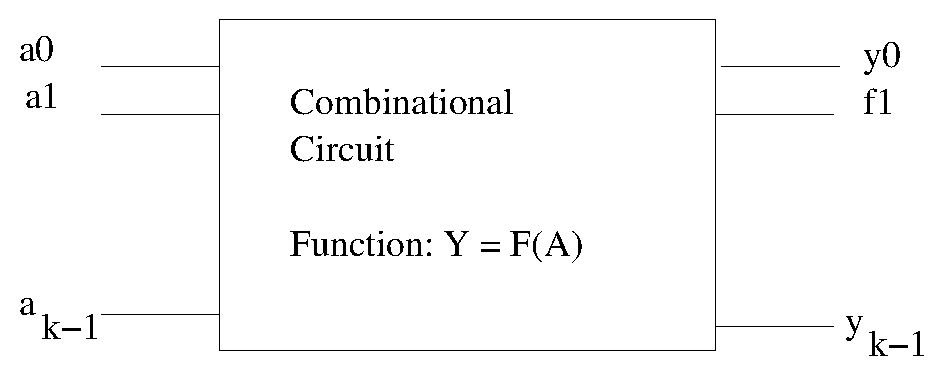
\includegraphics[scale=0.4]{interp.eps}
}


\begin{itemize}
\item Circuit: $f: \mathbb{B}^{k} \rightarrow \mathbb{B}^k$
\item $f: \Zkk \rightarrow \Zkk$ or ~~$f: \Zkk \rightarrow \Zkk$
\item Interpolate a polynomial from the circuit: $Y = F(A)$
\item $A = a_0 + a_1\alpha + \dots a_{k-1}\alpha^{k-1}, ~~Y = y_0 +
  y_1\alpha + \dots y_{k-1}\alpha^{k-1}$ 
\item Compute Gr\"obner basis of circuit polynomials with Elimination order:
  circuit-variables $> Y > A$
\item Obtain $Y = F(A)$ as a \alert{unique, canonical, polynomial}
  representation from the circuit
  
\end{itemize}




\end{frame}



\begin{frame}{\large Polynomial Interpolation from Circuits}

\centerline{
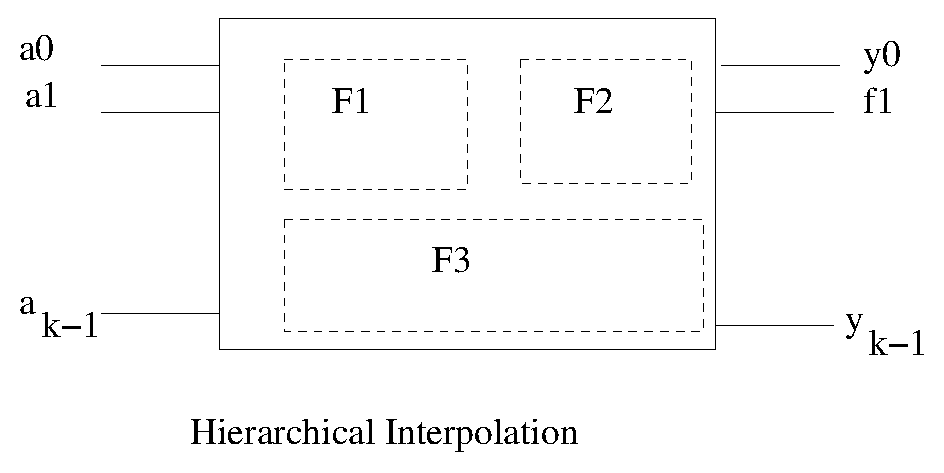
\includegraphics[scale=0.5]{h.eps}
}


\begin{itemize}
\item Partition the circuit into sub-circuits
\item Interpolate Polynomials $F_1, F_2, \dots$ from Partitions
\item Re-compute Gr\"obner basis of $\{ F_1, F_2, \dots \}$
\item Eliminate internal variables to obtain $Y = F(A)$   
\end{itemize}




\end{frame}


%%%%%%%%%%%%%%%%%%%%%%%%%%%%%%


\begin{frame}{\large{Conclusions}}


\begin{itemize}
\item Formal Verification of large Galois Field circuits
\item Computer algebra approach:
\begin{itemize}
	\item  Nullstellensatz+Gr\"obner Bases methods
	\item Engineering $\rightarrow$ a term order to obviate
          Gr\"obner basis computation
	\item Can verify upto $163$-bit circuits
          \item NIST specified $163$-bit field.... practical verification!
\end{itemize}
\item Our approach relies only on polynomial division
\item Complexity of polynomial division: Polynomial in the size of
  $f_1, \dots, f_s$
\item Almost the same time to catch bugs
\item Conventional approaches fail miserably.....
\item Future Work: Verify sequential GF-arithmetic Circuits
\begin{itemize}
\item State-space traversal: Quantifier Elimination over Gr\"obner Basis
\end{itemize}
\end{itemize}

\end{frame}
%%%%%%%%%%%%%%%%%%%%%%%%%%%%%%
\begin{comment}
\begin{frame}{Questions?}
\bigskip
\vspace{0.9in}
\hspace{1.5in}
Vielen Dank! \\
\bigskip
\hspace{1.5in}
Questions?
\end{frame}
\end{comment}
%%%%%%%%%%%%%%%%%%%%%%%%%%%%%%


\end{document}

